\documentclass[letterpaper]{ltxdoc}

\usepackage[hmargin={3 cm,3cm},top=1.5cm, marginpar=3cm]{geometry}
\usepackage{graphicx}
\usepackage{hyperref}
\hypersetup{colorlinks, linkcolor=blue, urlcolor=blue}
\usepackage{multicol}
\usepackage{lipsum}
\usepackage{xcolor}
\usepackage{pdfpages}
\usepackage{listings}
\definecolor{mauve}{rgb}{0.58,0,0.82}
\definecolor{dkgreen}{rgb}{0,0.6,0}
\lstdefinestyle{DOS}
{
backgroundcolor=\color{gray},
basicstyle=\color{white}\ttfamily,
breaklines=true,
postbreak=\mbox{\textcolor{red}{$\hookrightarrow$}\space}
}

\lstdefinelanguage{Cypher}
{
morekeywords={MATCH, WHERE, RETURN, CREATE, ORDER, BY, ITERATE, LOOP, ON, COLLECT, AS, AND, OR, DISTINCT,
ASC, DESC, LIMIT, SKIP, UNION, UNION, ALL, COUNT, FOREACH, WITH, NOT, count, collect, sum,
min, max, avg, id, IN, labels, exists},
morestring=[b]",
basicstyle={\small\ttfamily},
keywordstyle=\color{blue},
commentstyle=\color{dkgreen},
stringstyle=\color{mauve}\ttfamily,
comment=[l]//,
numbers=left,
xleftmargin=1em,
frame=single,
framexleftmargin=2em
}

\lstset{frame=tb,
language=Java,
aboveskip=3mm,
belowskip=3mm,
showstringspaces=false,
columns=flexible,
basicstyle={\small\ttfamily},
numbers=none,
numberstyle=\tiny\color{gray},
keywordstyle=\color{blue},
commentstyle=\color{dkgreen},
stringstyle=\color{mauve},
breaklines=true,
breakatwhitespace=true,
tabsize=3
}

\begin{document}
\title{\textsf{Cyp2SQL -- Documentation}}

\author{Oliver Crawford\\ojc37@cam.ac.uk}

\maketitle

\abstract{\emph{Cyp2SQL} is a tool for translating graph schemas and the graph query language Cypher to both
a different database schema, and different database language (the original aim of this project was to translate
Cypher to SQL). The tool can either be used as a standalone application, or, by utilising the .jar of the Java application, it can be used as an API for other applications. The license of the code is to be confirmed.}

\tableofcontents
\addtocontents{toc}{%
\protect\setlength{\columnsep}{5pc}
\protect\begin{multicols}{2}}

\section{Overview}

\begin{figure}[h]
\centerline{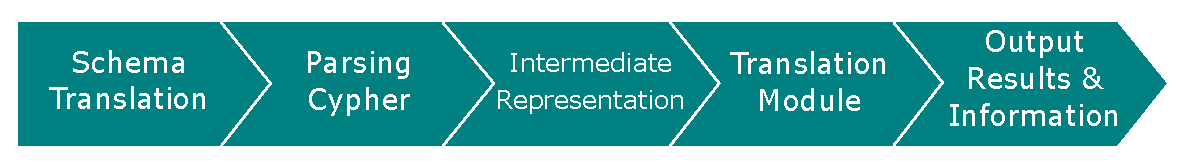
\includegraphics[width=\textwidth,height=\textheight,keepaspectratio]{toolchainVec.eps}}
\caption{The five stages of the pipeline.}
\label{toolchain}
\end{figure}

The pipeline of the tool consists of 5 stages (as shown in Figure \ref{toolchain}):

\begin{itemize}
\item A \emph{Schema Conversion} module for creating the initial database in a representation other than Neo4j (such as a relational schema in Postgres)
\item A \emph{Parsing Cypher} module, which is the first part of the translation to another database language (such as SQL). This module relies on the ANTLR framework, and other hand-written parsing code
\item An \emph{Intermediate Representation} is then built in Java -- the result of this stage of the pipeline is a \texttt{DecodedQuery} object.
\item A \emph{Translation Module} takes this intermediate representation, and converts it to the target database language
\item The \emph{Output Results \& Information} module can perform many different tasks, depending on the configuration desired:
\begin{itemize}
\item It can execute both the original Cypher on Neo4j, and the newly created query on the target database, and record the execution times of the queries. The tool may also be made to write the results to local files, so that the outputs can be compared for accuracy.
\item The tool can also just execute the translated query on the database engine, and parse the results back into the \emph{Cyp2SQL} tool.
\end{itemize}
\end{itemize}

\medskip

The codebase is entirely Java. There are some additional features provided through the ANTLR tool, as described in \S \ref{sec:antlr}. There are some script/.bat files that help the tool execute SQL on Postgres and pipe the results back into the tool.

\subsection{Quick usage}
Using the \texttt{cyp2sql-next.jar} file:
\begin{verbatim}
<-schema|-translate|-s|-t> <propertiesFile> <targetDatabaseName> <-dp|-dn|-r>
\end{verbatim}

\begin{center}
\begin{tabular}{ p{3cm} p{10.5cm} }
\texttt{-s \textbar{} -schema} & Runs the tool for schema conversion. See \S \ref{sec:schemaConv}. \\
\texttt{-t \textbar{} -translate} & Runs the tool for query translation. See \S \ref{sec:tranQ}. \\
\texttt{propertiesFile} & Path of the properties file \texttt{c2s\_props.properties}. See \S \ref{ss:prop}. \\
\texttt{targetDatabaseName} & Name of the relational database for either the converted graph schema to be stored into, or for the translated queries to execute on. \\
\texttt{dp \textbar{} -dn \textbar{} -r} & \textbf{Only needed when in query translation mode}.
\end{tabular}
\end{center}

\medskip

Using the code within another application as a library is also possible. Example usage:

\begin{lstlisting}[language=Java, breaklines=true]
import database.postgres.InsertSchemaPostgres;
import intermediate_rep.DecodedQuery;
import production.C2SMain;
import production.C2SProperties;
import schema_conversion.SchemaConvert;

import java.io.IOException;

public class C2STestUsage {
public static void main(String args[]) {
// these need to be set before anything can occur.
String propsFile = "C:/Users/ocraw/IdeaProjects/cyp2sql-next/c2s_props.properties";
C2SProperties props = new C2SProperties(propsFile);

// name of the blank database to either:
// - convert the schema too
// - execute the translated Cypher on
String dbName = "testb";

String thingToDo = "translate";

switch (thingToDo) {
case "convert":
// the properties file must be edited first.
// a dump from Neo4j is also needed.
boolean successConvert = SchemaConvert.translate(props);
if (successConvert) InsertSchemaPostgres.executeSchemaChange(dbName, props);
break;
case "translate":
// location of the script to allow results from Postgres to be
// piped back to this class. Adapt the scripts if necessary.
String scriptLoc = "C:/Users/ocraw/IdeaProjects/cyp2sql-next/pgdbPlay.bat";

// Cypher query to translate and then execute.
String cypher = "MATCH (a:Meta) RETURN DISTINCT a.type " +
"UNION MATCH (a:Process) RETURN DISTINCT a.type;";

try {
// obtain the intermediate representation
DecodedQuery dQ = C2SMain.getDQ(cypher, props);
System.out.println(dQ.getUnionParts().get(0).getMc());

// convert the intermediate representation to SQL
String sql = C2SMain.getTranslation(cypher, dQ, props);
System.out.println(sql);

// execute directly on Postgres if desired (the script will pipe
// the results back into this tool).
String postgresOutput = C2SMain.runPostgres(sql, dbName, scriptLoc);
System.out.println(postgresOutput);
} catch (IOException e) {
e.printStackTrace();
}
break;
default:
System.err.println("Not a valid option...");
System.exit(1);
}
}
}
\end{lstlisting}

\section{Getting started}
The code for the tool can be found in the \emph{cyp2sql-next} repository: \url{https://gitlab.dtg.cl.cam.ac.uk/fresco-projects/cyp2sql-next/}.

\medskip

There is an initial setup procedure involved before the tool can be run. View the \texttt{README.md} for additional information.

\medskip

\textcolor{red}{NOTE: Javadoc documentation is also available through the repo.}

\medskip

\textcolor{red}{NOTE: a .JAR file is included within the repo that can be run from the command line.}

\subsection{Prerequisites}
\begin{itemize}
\item Java 1.8 or above
\item Neo4j, any version should suffice
\item \textbf{An existing graph database} in Neo4j
\item A target database engine for the queries to be translated for, such as Postgres
\item Windows or Unix OS
\item For large databases, a relatively powerful machine and available disk space (additionally, as much RAM as possible)
\end{itemize}


\subsection{File system preparation}
The easiest way to use the tool is to create a new folder, and to also create/add the following folders/files:

\begin{itemize}
\item A folder for workspace usage
\begin{itemize}
\item Metafiles created during the schema conversion will be stored here
\end{itemize}
\item A blank text file for storing the keys of the graph that may contain lists -- see \S \ref{sssec:lists}
\item A folder for storing the results from both the Neo4j database, and the target database. For example, create a folder called \texttt{results}, and then two files within this folder called \texttt{results\textbackslash neo4jResults.txt} and \texttt{results\textbackslash postgresResults.txt}
\item A new Postgres database should also be created -- in Unix this can be done via the command \texttt{createdb <nameOfNewDatabase>}
\end{itemize}


\subsection{Generating dump files from Neo4j}
The tool builds up an equivalent schema in the target database by parsing a text file that is generated via the Neo4j console.

\medskip

\textcolor{red}{NOTE: the console/Java application offered by Neo4j is currently being deprecated in favour of the new `cypher-shell'.}

\medskip

\textcolor{red}{NOTE: the dump file may be very large for large graph databases.}

\subsubsection{Windows OS}
\begin{lstlisting}[style=DOS]
java -classpath "C:\Program Files\Neo4j CE 3.0.6\bin\neo4j-desktop-3.2.2.jar" org.neo4j.shell.StartClient -path "C:\Users\ocraw\Documents\CL Internship\Neo4j graphs\Test1KOPUS" -c dump > "C:\Users\ocraw\Documents\CL Internship\Graph Dumps\dumpOPUS1k.txt"
\end{lstlisting}

\subsubsection{Unix OS}
\begin{lstlisting}[language=bash, breaklines=true, postbreak=\mbox{\textcolor{red}{$\hookrightarrow$}\space}, backgroundcolor=\color{gray}, basicstyle=\color{white}\ttfamily]
neo4j-shell -path ../data/databases/dump_prov1000.graphdb/ -c dump > 2017-08-01-dump.txt
\end{lstlisting}


\subsubsection{Dump file explanation}
The dump file should look something like:

\begin{verbatim}
begin
commit
begin
create (_0:`Local` {`mono_time`:"10", `name`:"omega", `node_id`:1, `ref_count`:1, ...
create (_1:`Global` {`name`:["nginx"], `node_id`:2, `sys_time`:-782642514, `type`:2})
create (_2:`Global` {`name`:["nginx"], `node_id`:3, `sys_time`:-782642514, `type`:2})
\end{verbatim}

The tool will remove the unnecessary lines from the file, leaving two distinct types remaining to parse into a relational schema: nodes and edges (relationships).


\subsection{Configuring the properties}
\label{ss:prop}
The file \texttt{c2s\_props.properties} contains all the necessary parameters to allow the tool to function correctly. This file should be edited before running the tool.

\begin{center}
\begin{tabular}{ p{3cm} p{10.5cm} }
neo4jSchema & Path of the dump file generated from the existing Neo4j graph. \\
workspaceLocation & Path to workspace used by the tool. \\
neo4jResults & Path for the results from the Neo4j database to be stored into, when a Cypher query is executed. \\
sqlResults & Path for the results from the relational database to be stored into, when an SQL query is executed. \\
listsLocation & Path to the text file containing the list of fields that may contain lists. \\
neo4jUser & Neo4j graph database username. \\
neoPW & Neo4j graph database password. \\
postgresUser & Postgres database username. \\
postgresPW & Postgres database password. \\
\end{tabular}
\end{center}


\section{Schema conversion}
\label{sec:schemaConv}
The first step of the pipeline in translating Cypher to SQL is to convert the Neo4j graph database to a relational database. Using the dump file generated from the Neo4j graph, multiple relations can be built up and executed on a relational database backend. During this process, other metafiles are also created -- these are used throughout the translation process later for completeness, and in some cases, optimisations.


\subsection{Converting the graph database to a relational schema}
For the tool to run successfully and without error, make sure all the properties in the properties file are correct. Next, a blank relational database needs to be created. The tool currently will not overwrite existing databases -- if an error has occurred when writing to the database, it must be wiped clean before the tool can run again.

\medskip

\begin{verbatim}
-s C:\Users\ocraw\IdeaProjects\Cypher_SQL_Translation\c2s_props.properties testDB
\end{verbatim}

\medskip

\begin{itemize}
\item The first argument (\texttt{-s}) signals to the program that it should be performing the schema conversion
\item The second argument is the location of the properties file
\item The third argument is the name of the recently created blank database
\end{itemize}

\medskip

If the tool runs successfully and without error, the following should have happened:

\begin{itemize}
\item The recently created database will now be populated with tables and data -- see \S \ref{ssec:grreltheory}
\item The workspace folder will now contain four metafiles -- see \S \ref{ssec:meta}
\end{itemize}

\medskip

\textcolor{red}{NOTE: deleting the workspace folder and its metafiles will cause some translations to fail. If this is done accidentally, the whole graph schema must be converted again from scratch.}


\subsection{Graph to relational: theory}
\label{ssec:grreltheory}
All the nodes from the graph are stored in one relation (nodes), and all the relationships are stored in a separate relation (edges).

There are some optimisations and additional implementation aspects. Storing all the attributes of the nodes in one relation, where there are multiple labels, will lead to a lot of NULL values populating the relation. To combat this, each individual label also has its own relation. The translator tool decides at run time the optimal relation to join.

Furthermore, each relationship type has its own relation. Although this optimisation is quicker, the trade-off will be roughly double the amount of disk space required to store all the relations, as well as the additional complexity in the translation tool.

For graph functions to be computable on the relational side, the schema converter also builds two materialised views –- \texttt{adjlist\_from} \& \texttt{adjlist\_to}.

Some other functions are also committed to the database at this point:

\begin{center}
\begin{tabular}{ p{4.5cm} p{9cm} }
\texttt{array\_unique(arr anyarray)} & Helper function for the \texttt{cypher\_iterate} function (see below). This function takes an array of any type as input, and returns an array of the same type, but with duplicate elements removed. \\

\texttt{cypher\_iterate(integer[])} & Function for performing the iterate function designed for this project. \\

\texttt{doforeachfunc(integer[], field TEXT, newv TEXT)} & Function to help perform the semantics of Cypher’s \texttt{FOREACH} keyword.
\end{tabular}
\end{center}

\medskip

\textcolor{red}{NOTE: the class \texttt{PostgresConstants.java} contains the list of additional materialised views and functions committed to the database during the schema conversion process.}

\medskip

Figure \ref{schemaConv} shows in detail an example conversion (the example is based on an OPUS graph with 100{,}000 nodes).

\begin{figure}[p]
\centerline{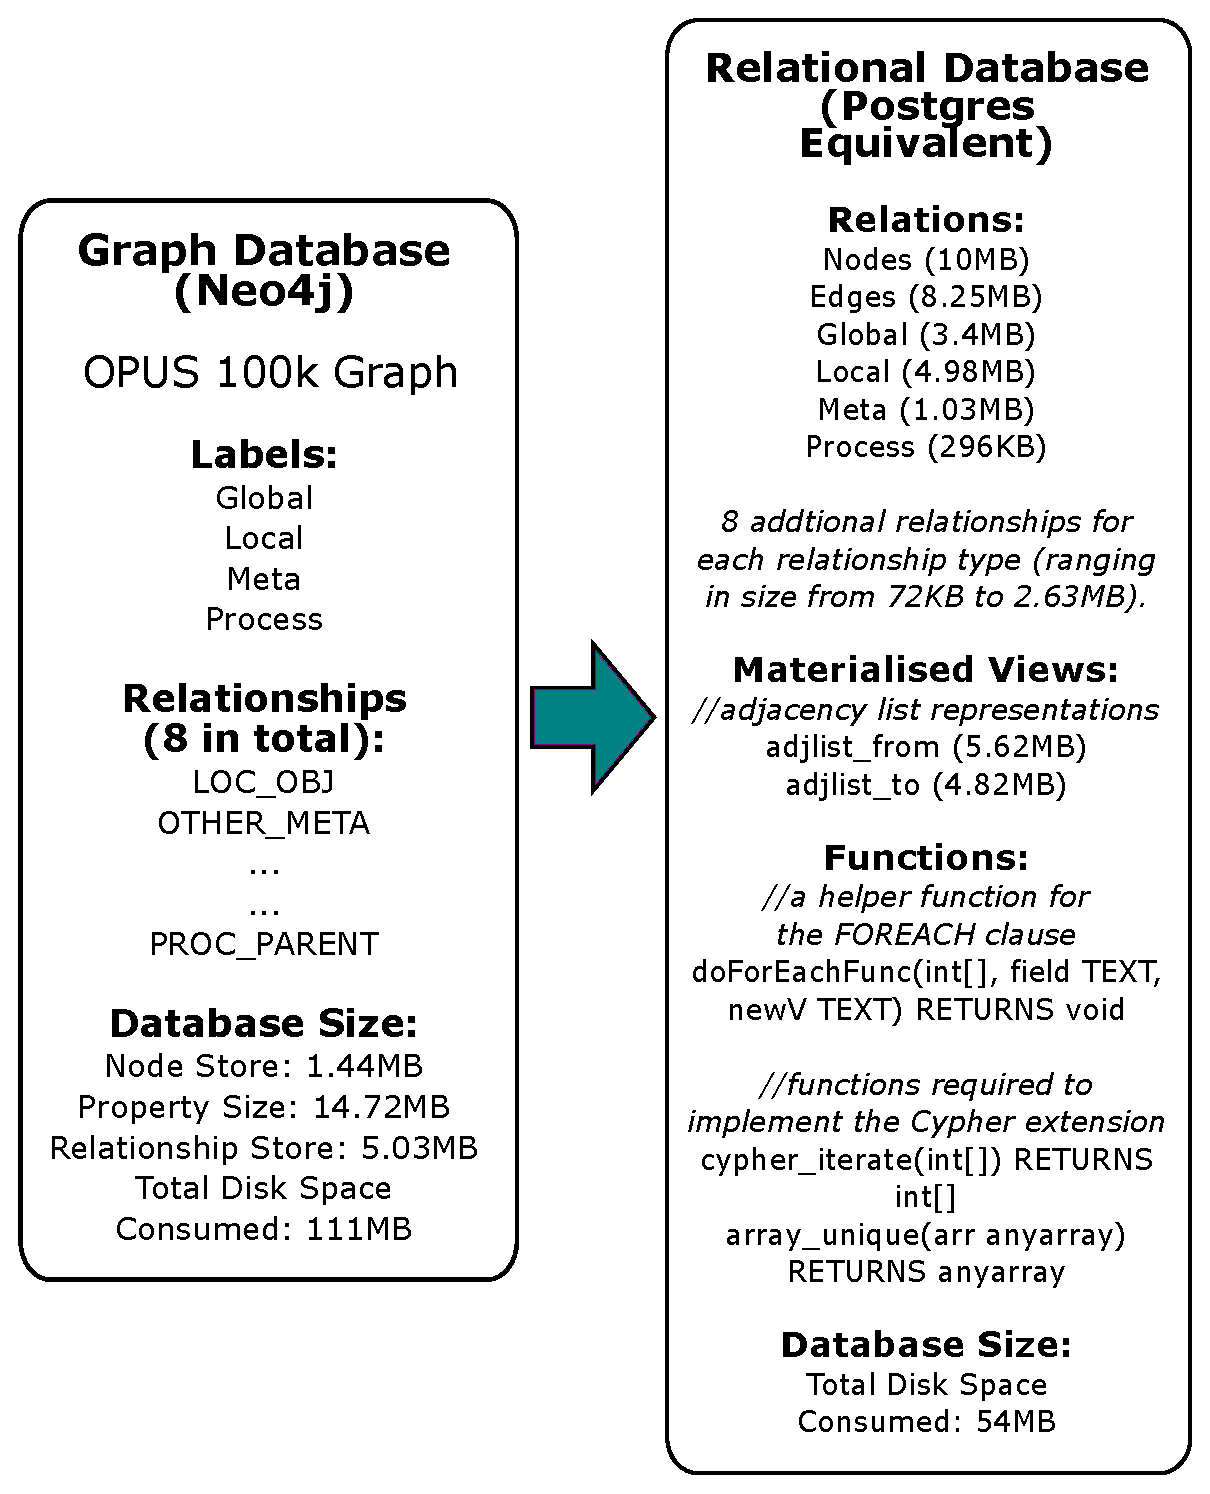
\includegraphics[width=\textwidth,height=\textheight,keepaspectratio]{schemaConv.eps}}
\caption{Schema conversion outline.}
\label{schemaConv}
\end{figure}

\subsection{Metafiles created during schema conversion}
\label{ssec:meta}
\texttt{meta\_nodeProps.txt} -- \textbf{Creation:} all properties of the nodes are stored in this file. \textbf{Usage:} currently two major uses. One is to help the Neo4j database driver to return the correct results to the user (for example, when a wildcard is used in the query). Secondly, it is used in the cases where a GROUP BY is required in the SQL statement to be executed.

\bigskip

\texttt{meta\_labelProps.txt} -- \textbf{Creation:} a slightly more detailed version of the file above. The file contains the list of properties of all the nodes, but is sectioned into the individual label types of the nodes.

Example:
\begin{verbatim}
*country*
name
population
dialling_code
*city*
name
population
state
ave_house_price
\end{verbatim}

\textbf{Usage:} the file is used to see if any possible optimisations to the SQL query are achievable. This is done by finding unique nodes for a property. In the example above, if the property/key `state' only belongs to the label `city', then the tool can use this information to its advantage.

See the method \texttt{getLabelMapping()} in \texttt{C2SMain.java} for further information. Information from this file is stored in the \texttt{labelProps} map (publicly accessible using \texttt{C2SMain.labelProps}).

\bigskip

\texttt{meta\_rels.txt} -- \textbf{Creation:} all the types of edges in the Neo4j graph are stored in this file.
\textbf{Usage:} currently only used in the case where the tool can be used to delete information from the database (this feature has not been thoroughly tested yet though, so caution is advised if a query which is being used to delete data is to be executed).

See the method \texttt{getLabelMapping()} in \texttt{C2SMain.java} for further information. Information from this file is stored in the \texttt{allRelTypes} map (publicly accessible using \texttt{C2SMain.allRelTypes}).

\bigskip

\texttt{meta\_labelNames.txt} -- \textbf{Creation:} all the names of the labels in the Neo4j graph are stored.
\textbf{Usage:} another optimisation technique -- helps the tool choose the best relation to use to complete the query correctly.


\section{Translation of queries}
\label{sec:tranQ}
\subsection{Usage}
The tool requires a running Neo4j instance to be up and running.

\medskip

\begin{verbatim}
-t \..\..\c2s_props.properties testDB <-dp|-dn|-r>
\end{verbatim}

\medskip

\begin{itemize}
\item The first argument (\texttt{-t}) signals to the program that it should be performing the translation of queries
\item The second argument is the location of the properties file
\item The third argument is the name of the relational database that the queries are to be executed on
\item The fourth argument is another flag that gives the user some choice in what they want to do -- see the table below for further guidance
\end{itemize}

\begin{center}
\begin{tabular}{ p{2cm} p{11.5cm} }
\texttt{-dp or -dn} & \textbf{Debug interface}. This function allows the user to input queries through the command line interface for translation. Useful for debugging. If \texttt{-dp} is used, the results from both the databases are printed to local files. If \texttt{-dn} is set, this does not occur. \\

\texttt{-r} & \textbf{Run as normal}. This function allows the user at the command line to input queries for translation. Unlike \texttt{-dp} or \texttt{-dn}, this will not execute Cypher on Neo4j, and will only output the results from the target database engine.
\end{tabular}
\end{center}

\medskip

\textcolor{red}{NOTE: the script to run Postgres on Unix systems when the tool is in \texttt{-r} mode may not have the right permissions to run with the tool. \texttt{chmod +x auto\_run\_pg.sh} should fix the issue.}

\medskip

The user at this point should be presented with a command line interface where Cypher can be typed into:

\begin{figure}[h]
\centerline{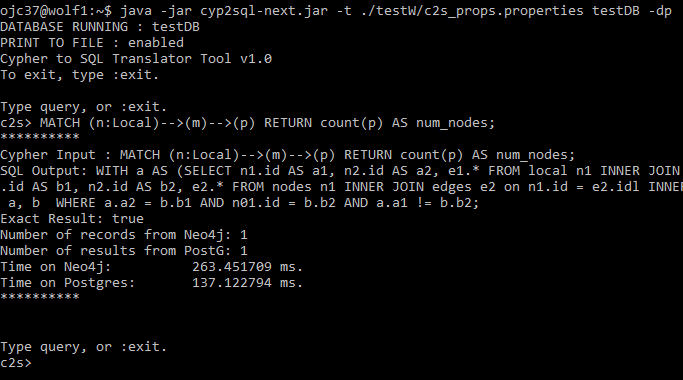
\includegraphics[width=\textwidth,height=\textheight,keepaspectratio]{ss1.png}}
\caption{Screenshot of debug mode.}
\label{ss1}
\end{figure}

\begin{figure}[h]
\centerline{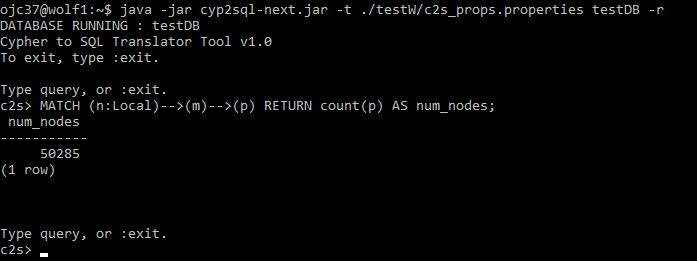
\includegraphics[width=\textwidth,height=\textheight,keepaspectratio]{ss2.png}}
\caption{Screenshot of run mode.}
\label{ss2}
\end{figure}


\subsection{Query translation}
The query is first tokenised using the ANTLR generated classes for the Cypher language. See \S \ref{sec:antlr} for more details.

An intermediate representation in the form of a DecodedQuery object is the built. This object is then referred to when translating to the target language (such as SQL). See \S \ref{ssec:workflow} for more detailed descriptions.

Multiple different classes can be used to perform the translation to SQL. Likewise, if a new type of translation is needed, the \texttt{AbstractConversion.java} and \texttt{AbstractTranslation.java} classes can be extended to suit.

\subsubsection{Dealing with Cypher lists}
\label{sssec:lists}
Lists in Cypher present one current challenge for the translation tool. Although the translation can be done, there is no current mechanism for detecting cleanly which keys of nodes/relationships may have type list.

To solve this problem (and to possibly fix any issues encountered with lists), a blank file should be created (with a name such as \texttt{lists.txt}). This file should then be referred to in the \texttt{c2s\_ props.properties} file (see \S \ref{ss:prop}).

The file should contain a list, separated by new lines, of each possible key in the graph that may contain a list. This will aid the translator in producing the correct result.


\subsubsection{Where clauses}
Where clauses are converted into properties of nodes/relationships. For example, if there is a Cypher clause, \texttt{MATCH (n) WHERE n.a = 1 AND n.b = 2 RETURN n}, then the translator tool associates the two predicates to the node \texttt{n}. When the translation to SQL occurs, the properties of node \texttt{n} are then extracted and converted.

The whole where clause is decoded in \texttt{CypherTranslator.java}. The initial clause is separated into its individual parts (they will be separated by either AND/OR). A \texttt{CypWhere} object is then created for each component, to store:

\begin{itemize}
\item The position it appears in the clause (the indexing counting left to right)
\item Any brackets that appear before or after the clause (to ensure consistent ordering later)
\item The boolean operator that immediately follows it
\end{itemize}

Depending on what the clause itself is conveying, it is parsed accordingly. When it has been parsed, the properties and semantics need to be stored. As mentioned above, they are stored with the nodes/relationships that they belong with. For example, if the where clause says something like \texttt{a.name = `me'}, the properties and semantics of the clause will be stored with the node that has the id \texttt{`a'} (assuming \texttt{`a'} is of course a node and not a relationship).

The format of how it is stored with the nodes/relationships is initially quite confusing (and in all honesty a bit silly, could do with a refactor), but can be quickly described with this guide:

\bigskip

\begin{lstlisting}[language=Cypher]
MATCH p=shortestPath((f {name:"omega"})-[*1..6]->(t:Meta))
RETURN count(t);
\end{lstlisting}

Property stored with node: \texttt{[name="omega"]}

In this example, as the property is described within the node itself, the property is simple to understand and parse.

\bigskip

\begin{lstlisting}[language=Cypher]
MATCH (a:Meta)
WHERE a.sys_time < 0
RETURN count(a);
\end{lstlisting}

Property stored with node: \texttt{[sys\_ time="p1null@null\$lt\#0\#tl"]}

\begin{itemize}
\item Already, the syntax looks very different, but can be broken down easily
\item \texttt{p1} denotes that the component \texttt{a.sys\_time < 0} is in the first position of the clause (in fact, in this example, it is the only component)
\item The \texttt{null} before the @ symbol means there is no boolean operator (such as AND or OR) that follows this component
\item The \texttt{null} after the @ symbol means that the component is not associated with any bracketing
\item The value after the \$ sign, \texttt{lt\#0\#tl} describes the predicate itself:
\begin{itemize}
\item \texttt{lt} is the code for the \texttt{<} symbol
\item The operand 0 is contained within the \# symbols
\end{itemize}
\end{itemize}

\bigskip

\begin{lstlisting}[language=Cypher]
MATCH (a)
WHERE a.node_id < 345
OR (
(a.node_id > 800 AND 'Process' in labels(a))
OR a.node_id = 983
)
RETURN count(a);
\end{lstlisting}

Property stored with node:
\texttt{[node\_id="p1or@null\$lt\#345\#tl\textasciitilde p2and@((\$gt\#800\#tg\textasciitilde p4null@)\$eq\#983\#qe", label="p3or@)\$eq\#process\#qe"]}

\begin{itemize}
\item In this case, two fields of the node have properties associated with them
\item When multiple properties apply to one field, the \textasciitilde {} symbol separates the individual components that will be translated
\item When brackets are involved (notice in the original Cypher input the 2 left brackets before \texttt{a.node\_id > 800}), these are stored after the @ symbol (in their literal form)
\begin{itemize}
\item Extra care must be taken in the code in the case of functions such as \texttt{labels(a)} at the end of a component (only one bracket should be recorded and not two)
\end{itemize}
\end{itemize}

\begin{center}
\begin{tabular}{ p{2.5cm} p{11cm} }
\texttt{eq\#...\#qe} & Equality: \texttt{WHERE idA.property = someValue}. \\
\texttt{ne\#...\#en} & Not equal to: \texttt{WHERE idA.property <> someValue}. \\
\texttt{lt\#...\#tl} & Less than: \texttt{WHERE idA.property < someValue}. \\
\texttt{gt\#...\#tg} & Greater than: \texttt{WHERE idA.property > someValue}. \\
\texttt{le\#...\#el} & Less than or equal to: \texttt{WHERE idA.property <= someValue}. \\
\texttt{ge\#...\#eg} & Greater than or equal to: \texttt{WHERE idA.property >= someValue}. \\
\texttt{ex\#...\#xe} & Exists function: \texttt{WHERE exists(idA.property)}. \\
\texttt{nx\#...\#xn} & Exists function (not): \texttt{WHERE not exists(idA.property = someValue)}. \\
\texttt{in\#...\#ni} & IN: \texttt{WHERE `someLabel' in labels(idA)}. \\
\texttt{anyin\#...\#niyna} & Any (where IN is also used): \texttt{WHERE any(var IN idA.property WHERE var IN [someList]}. \\
\texttt{anyeq\#...\#qeyna} & Any (where IN is also used): \texttt{WHERE any(var IN idA.property WHERE var = someValue}. \\
\texttt{isn\#...\#nsi} & IS NULL: \texttt{WHERE idA.proeprty IS NULL}. \\
\texttt{non\#...\#non} & IS NOT NULL: \texttt{WHERE idA.proeprty IS NOT NULL}.
\end{tabular}
\end{center}


\subsubsection{Iterate semantics}
\label{sssec:iterate}
As part of an extension to my original dissertation on this tool, additional functionality to the graph model was included. The additional feature is looking at querying repeating patterns within a graph. A user defines a pattern they wish to search, and a schema for how to perform the iterative matching. The query will store all the nodes “touched” by the query, returning them similarly to traditional Cypher queries.

To make the extension simple, it was important to define the syntax in a clear and distinct manner, as demonstrated below:

\begin{lstlisting}[language=Cypher]
ITERATE MATCH (a {host: `google'})-->(b:Website)
-->(c {domain: `net'})
LOOP c ON b COLLECT n
RETURN n.host
\end{lstlisting}

The \texttt{ITERATE} keyword makes it both clear that the Cypher will attempt to iterate over a graph, and it is used as a flag for the tool, so that it can expect to parse the query correctly. The remaining syntax encompasses the iterate pattern: \texttt{LOOP (1) ON (2) COLLECT (3)}.

\texttt{(1)} is the node ID holding the results of intermediate queries. \texttt{(2)} marks the starting point in the query for the previous results to start from. \texttt{(3)} is an extra identifier that is separate from the main query, and is what is used in the \texttt{RETURN} clause.

To demonstrate what this new syntax can do, consider the graph in Figure \ref{iterGraphFig}.

Figure \ref{iterGraphFig} shows a common pattern, \texttt{BLUE --> GREEN --> RED --> BLUE}. Finding all the blue nodes at the end of this pattern \emph{iteratively} would be hard to do with the existing Cypher syntax in a concise and clear manner. It is a more tractable problem with the \texttt{ITERATE} syntax:

\begin{lstlisting}[language = Cypher]
ITERATE MATCH (a:l1)-->(b:l2)-->(c:l3)-->(d:l1)
LOOP d ON a COLLECT n
RETURN n.uid;
\end{lstlisting}

\begin{figure}[h]
\centerline{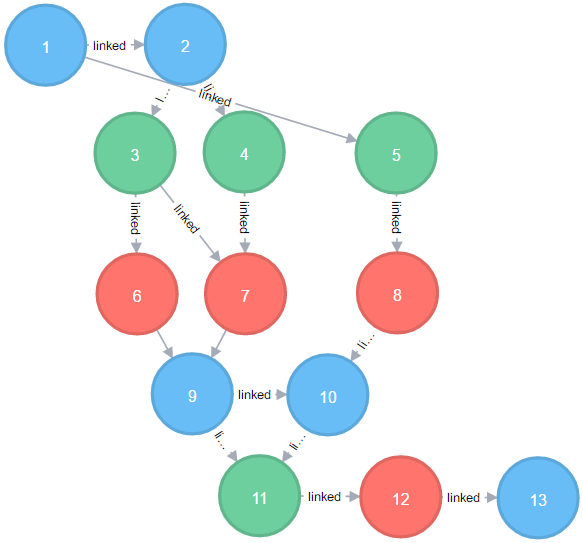
\includegraphics[scale=0.7]{iterateGraph.png}}
\caption{A trivial graph consisting of thirteen nodes with three different labels -- blue for `l1', green for `l2', and red for `l3'.}
\label{iterGraphFig}
\end{figure}

\newpage

Executing this query on Postgres returns the results shown in Table \ref{table:queryIter}.

\begin{table}[!h]
\caption{Results of Iterate Query.} % title of Table
\centering % used for centering table
\begin{tabular}{c} % centered columns (4 columns)
\hline\hline %inserts double horizontal lines
n.uid \\ [0.5ex] % inserts table
%heading
\hline % inserts single horizontal line
9 \\
9 \\
9 \\
10 \\
13 \\
13 \\
13 \\
13 \\ [1ex] % [1ex] adds vertical space
\hline %inserts single line
\end{tabular}
\label{table:queryIter} % is used to refer this table in the text
\end{table}

In comparison, running just the \texttt{MATCH} query on Neo4j once will return only six results. The extra two results that the \texttt{ITERATE} extension finds comes from the fact that the nodes with ID `9' and `10' are being used in another iteration of the \texttt{MATCH} clause. Hence the node with ID `13' is returned a further two times.

\subsection{Workflow through the code}
\label{ssec:workflow}
On the following pages is an example of how a query is translated from Cypher to SQL through the tool. Included with the flow are descriptions to help the reader.

\newpage
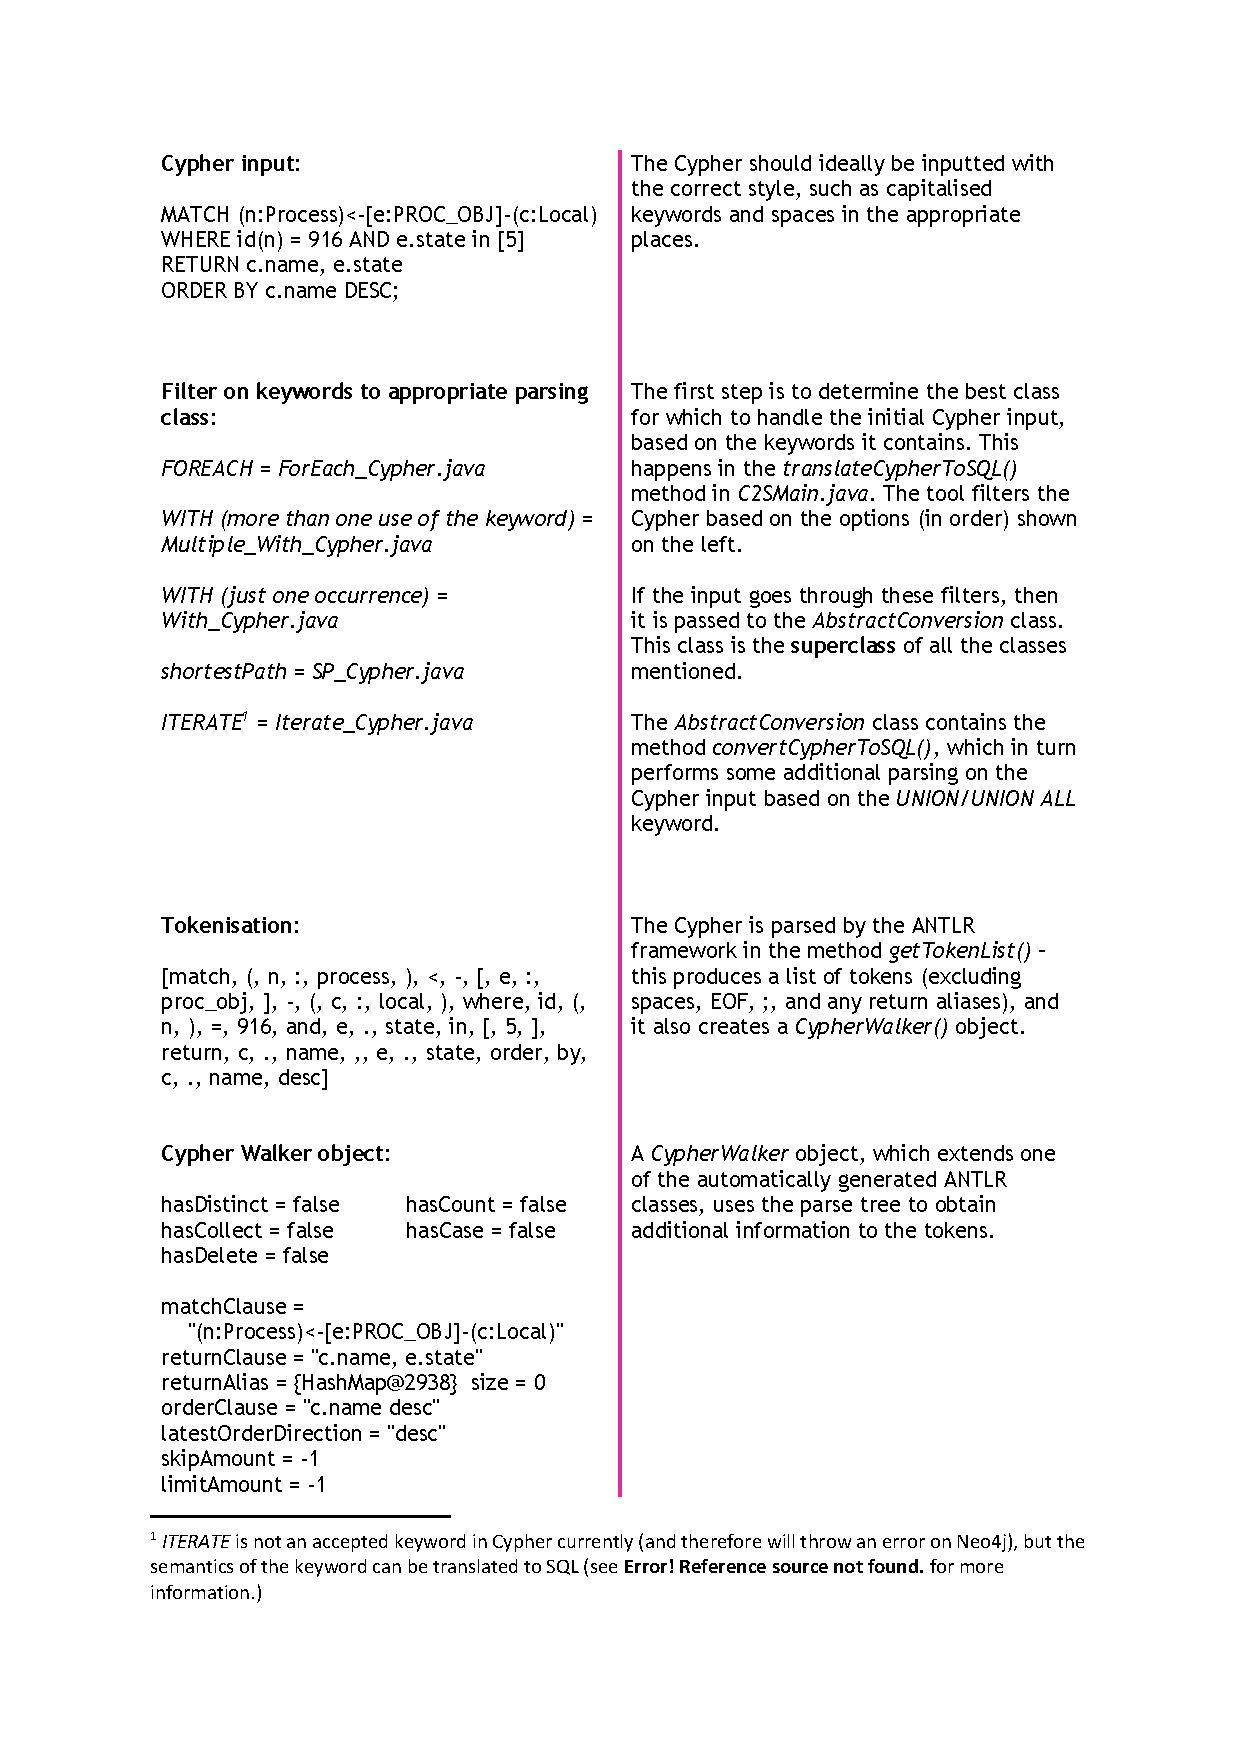
\includepdf[pages={-}]{workflow.pdf}


\section{ANTLR framework}
\label{sec:antlr}
The current tool uses ANTLR v4\footnote{\url{http://www.antlr.org/download.html}} as a way of parsing the initial Cypher query, both into tokens and as a more effective way of parsing information out of the query. The ANTLR framework requires a grammar of Cypher to work, and this has been obtained from the \emph{openCypher} project\footnote{\url{https://s3.amazonaws.com/artifacts.opencypher.org/M06/Cypher.g4}}.

The guide for setting up the parsers and lexers has been adapted from the ANTLR v4 `Getting Started' guide\footnote{\url{https://github.com/antlr/antlr4/blob/master/doc/getting-started.md}}.

\medskip

\textcolor{red}{NOTE: the parser and lexer should already be working and configured within the \emph{Cyp2SQL} code itself. The information below would be useful in the case of an update to either the Cypher grammar file, or to the ANTLR library. See the package \texttt{parsing\_lexing} for the existing configuration.}

\begin{figure}[h]
\centerline{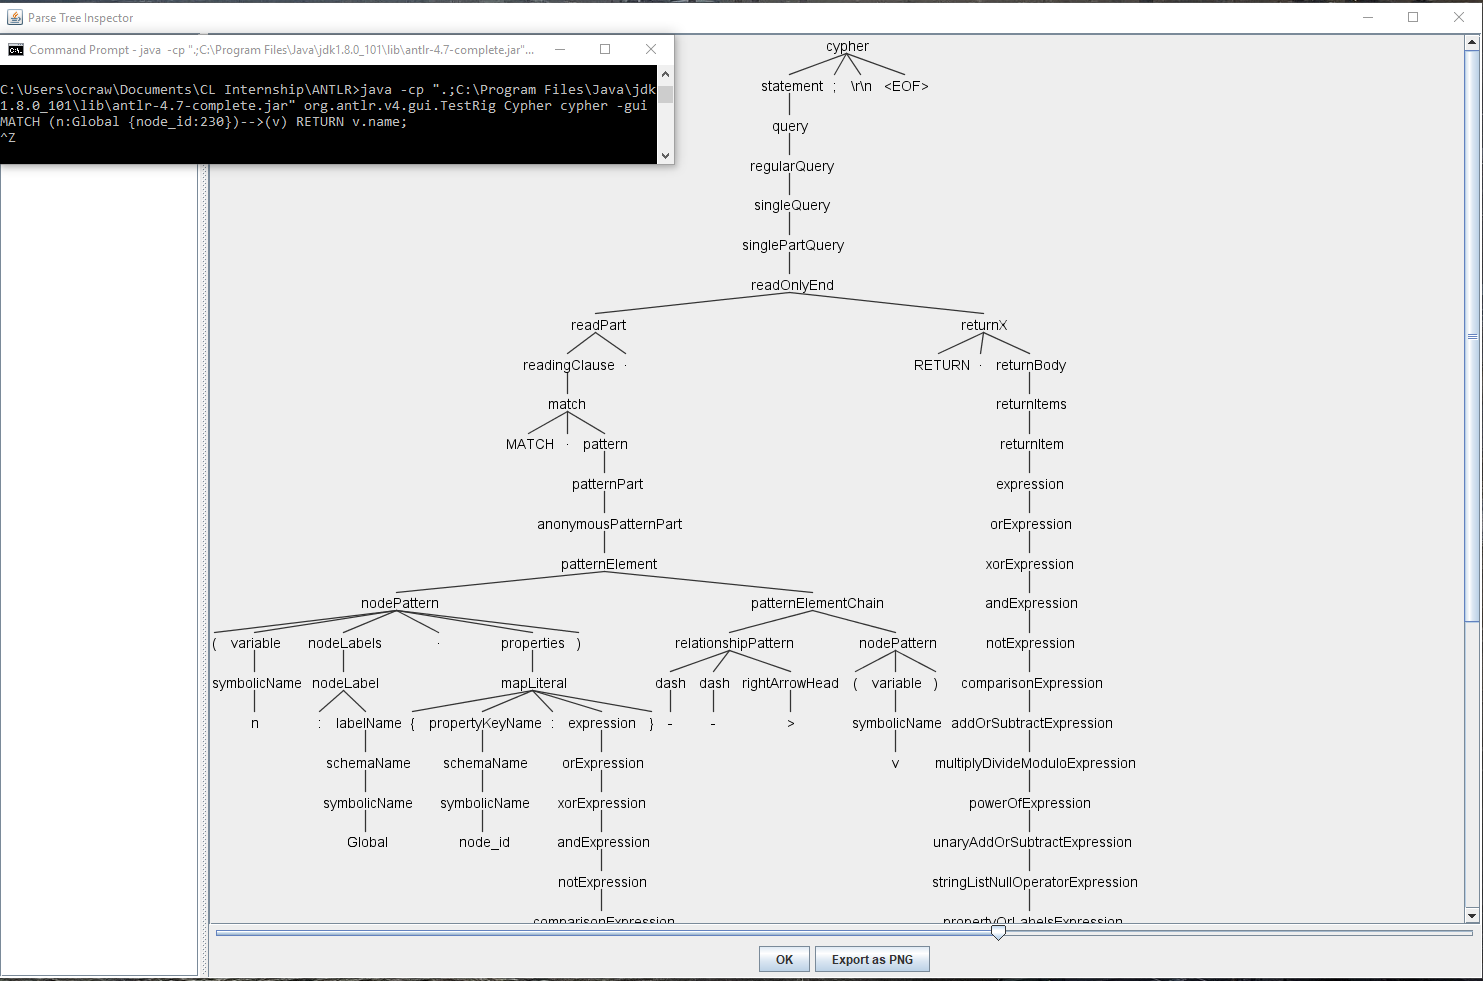
\includegraphics[width=\textwidth,height=\textheight,keepaspectratio]{ss3.png}}
\caption{Parse tree of a Cypher query with ANTLR.}
\label{antlrs}
\end{figure}

\subsection{ANTLR setting up}

Firstly, a new temporary folder should be made -- add to it the latest \texttt{Cypher.g4} grammar file.\footnote{One of the keywords in the original file was named \texttt{return}, but this clashes with the tool, and so it has been renamed to \texttt{returnX}} Then run the following command:

\begin{lstlisting}[style=DOS]
java -jar "C:\Program Files\Java\jdk1.8.0_101\lib\antlr-4.7-complete.jar" Cypher.g4
\end{lstlisting}

Followed by this command:

\begin{lstlisting}[style=DOS]
javac -classpath .;"C:\Program Files\Java\jdk1.8.0_101\lib\antlr-4.7-complete.jar" Cypher*.java
\end{lstlisting}

It is a good idea to test the installation at this point:

\begin{lstlisting}[style=DOS]
java -cp ".;C:\Program Files\Java\jdk1.8.0_101\lib\antlr-4.7-complete.jar" org.antlr.v4.gui.TestRig Cypher cypher -gui
\end{lstlisting}

Assuming a valid installation, commands can now be typed into the console - \texttt{\^{}Z} will end the input and hopefully produce an image, such as the one in Figure \ref{antlrs}.

The source code files generated by the tool are contained within the package \texttt{parsing\_lexing}.

\section{Current Cypher translation list}
The tool cannot currently translate the complete set of Cypher available to use. Below is a detailed guide of what can be translated. Further translations are more than possible by viewing/adapting the source code to suit.

\medskip

\textcolor{red}{NOTE: information gathered below has been adapted from the full list of Cypher commands obtained from the Neo4j Cypher reference card: \url{https://neo4j.com/docs/cypher-refcard/current/}}

\medskip

\textcolor{red}{NOTE: quantifiers from regular expressions may be used below to make the list more concise. As a quick reference, ${*}$ = zero or more times; + = one or more times; ? = zero or one time.}

\medskip

\subsection*{\texttt{MATCH ... RETURN ...}}
The queries below will be translated via the \texttt{NoRels.java} class.

\medskip

\begin{lstlisting}[language = Cypher]
MATCH (idA)
RETURN [DISTINCT]? idA

MATCH (idA:labelA)
RETURN idA.propertyA

MATCH (idA:labelA:labelB {keyA:valueA})
RETURN idA.propertyA AS alias_value, idA.propertyB AS other_alias

MATCH (idA)
RETURN [count(idA)|collect(idA.propertyA)|sum(idA.propertyA)|
min(idA.propertyA)|max(idA.propertyA)|avg(idA.propertyA)]
\end{lstlisting}

\subsection*{\texttt{ORDER BY, SKIP, and LIMIT}}
Queries containing these keywords need only a small adjustment to translate.

\medskip

\begin{lstlisting}[language = Cypher]
MATCH (idA)
RETURN idA.propertyA
ORDER BY idA.propertyB [ASC|DESC]?
[SKIP skipValue]? [LIMIT limitValue]?
\end{lstlisting}

\newpage

\subsection*{\texttt{MATCH ... WHERE ... RETURN}}
These are also translated to SQL in the class \texttt{NoRels.java}.

\medskip

\begin{lstlisting}[language = Cypher]
MATCH (idA)
WHERE [NOT]? idA.propertyA [=|<>|<|>|<=|>=] value
RETURN count(idA)

MATCH (idA)
WHERE idA.propertyA < valueA [AND|OR] idB.propertyB > valueB
RETURN count(idA)
\end{lstlisting}

\subsection*{Paths -- \texttt{MATCH ()-->()-->() ...}}
These are translated to SQL in the class \texttt{MultipleRel.java}.

\medskip

\begin{lstlisting}[language = Cypher]
MATCH (idA)-->(idB)-->(idC)-->(idD)
WHERE id(idD) < some_value
RETURN count(idA) AS some_alias

MATCH (idA)<-[[relID]?:REL_TYPE]-(idB)
RETURN idB
ORDER BY idB.propertyA ASC

MATCH ()-[r:REL_TYPE {keyA:valueA}]-()
RETURN r.propertyA
\end{lstlisting}

\subsection*{With -- \texttt{... WITH ... RETURN}}
These are translated to SQL in the class \texttt{WithSQL.java}, although additional parsing of the Cypher input will also occur in either the class \texttt{With\_Cypher.java} or \texttt{Multiple\_With\_Cypher.java}.

\medskip

\begin{lstlisting}[language = Cypher]
MATCH (idA:labelA)-[rel]->(idB:labelB)
WITH idA, count(rel) AS alias
WHERE alias > value
RETURN idA.propertyA, alias
ORDER BY alias DESC

MATCH (idA)
WITH idA
ORDER BY idA.propertyA DESC
LIMIT 3
RETURN collect(idA.propertyA)

MATCH (idA)
WHERE someLabel IN labels(idA)
WITH idA
MATCH (idB)
WHERE idB.propertyB = idA.propertyA
RETURN count(idA)
\end{lstlisting}

\newpage

\subsection*{\texttt{UNION [ALL]?}}
The individual components of the input are dealt with normally, and then combined together with the correct \texttt{UNION} semantics in the class \texttt{UnionSQL.java}.

\medskip

\begin{lstlisting}[language = Cypher]
MATCH (idA)-[:rel1]->(idB)
RETURN idB.propertyA
[UNION|UNION ALL]
MATCH (idA)-[:rel2]->(idB)
RETURN idB.propertyA
\end{lstlisting}

\subsection*{Variable length paths -- \texttt{-[*x..y]->}}
This subset of Cypher is dealt with using the \texttt{SingleVar.java} class.

\medskip

\begin{lstlisting}[language = Cypher]
MATCH (idA:labelA)-[*x..y]->(idB:labelB)
RETURN count(idB)

//x and y represent integer values for the length of the path
//being traversed. These queries, unlike the paths shown earlier,
//only currently work for one pattern - it cannot be extended
//in the following way:

MATCH (idA:labelA)-[*x..y]->(idB:labelB)-[*x2..y2]->(idC)
RETURN count(idC)

//furthermore, a direction must be specified.
\end{lstlisting}

\subsection*{Shortest path queries}
This subset of Cypher is dealt with using the \texttt{ShortestPath.java} class.

\medskip

\begin{lstlisting}[language = Cypher]
MATCH p=shortestPath((idA {key:value})-[*1..x]->(idB:labelB))
RETURN count(idB)
\end{lstlisting}

\subsection*{Functions -- \texttt{exists(), labels(), id()}}
These keywords are parsed in the class \texttt{CypherTranslator.java}, where they are stored with the node/relationship that they are referring to.

\medskip

\begin{lstlisting}[language = Cypher]
MATCH (idA)
WHERE exists(idA.propertyA) AND exists(idA.propertyB)
RETURN count(idA)

MATCH (idA)-[rel]->(idB)
WHERE NOT id(idB) = value OR "someLabel" IN labels(idB)
RETURN idA.propertyA
\end{lstlisting}

\newpage

\subsection*{\texttt{... WHERE ... IN} and \texttt{any()}}
These keywords are parsed in the class \texttt{CypherTranslator.java}, where they are stored with the node/relationship that they are referring to.

\medskip

\begin{lstlisting}[language = Cypher]
MATCH (idA)
WHERE id(idA) IN [val1, val2, ..., valN]
RETURN idA.propertyA

MATCH (idA)
WHERE any(someV IN labels(idA) WHERE someV IN [val1, ..., valN])
RETURN count(idA)

MATCH (idA)
WHERE any(someVar IN idA.propertyA WHERE someVar = value)
RETURN count(idA)
\end{lstlisting}

\subsection*{\texttt{ITERATE MATCH ...}}
This additional keyword is parsed and translated in the class \texttt{Iterate\_Cypher.java}. See \S \ref{sssec:iterate} for more details.

\medskip

\begin{lstlisting}[language = Cypher]
ITERATE MATCH (idA)-->(idB)-...->(idX)
LOOP idX ON idA COLLECT idN
RETURN idN.propertyA
\end{lstlisting}

\subsection{Known issues}
\begin{itemize}
\item The use of \texttt{WITH} is still quite constrained in its use
\item When predicates in the \texttt{WHERE} clause are added, they may sometimes lead to incorrect translations (mostly in the \texttt{WITH} parts of a multiple relationship Cypher input). It can be solved in some cases by adding the predicates in a different way in the original input (see example below)
\end{itemize}

\begin{lstlisting}[language = Cypher]
MATCH (a)-[e]->(b)-[f]->(c)
WHERE a.type = b.type AND c.pid < b.pid
RETURN count(f);

// instead of

MATCH (a)-[e]->(b)-[f]->(c)
WHERE a.type = b.type AND b.pid > c.pid
RETURN count(f);

// where 'b' now has 2 properties associated with it,
// and will not work (currently).
\end{lstlisting}

\subsection{List of test queries from OPUS}
\begin{verbatim}
MATCH p=shortestPath((f {name:"omega"})-[*1..6]->(t:Meta)) RETURN count(t);

MATCH (a)-[*1..3]->(c:Process) RETURN count(c);

MATCH (a:Local)-[*4..9]->(b)
RETURN DISTINCT b.node_id, b.sys_time AS time_alias ORDER BY b.node_id DESC;

MATCH (n {name:["/var/db/entropy/saved-entropy.7", "/var/db/entropy/saved-entropy.8"]})
RETURN n.node_id ORDER BY n.node_id ASC;

MATCH (a:Global)-[]->(b) RETURN b.node_id AS conn_id;

MATCH (a:Global)-[]->(b) RETURN count(b.node_id);

MATCH (a:Global)-->(b:Local)-->(c:Process)<--(d:Local)<--(b) RETURN count(b);

MATCH ()-[r]-() RETURN DISTINCT r.state ORDER BY r.state;

MATCH (n:Local)<--(m:Global)
RETURN m.node_id AS thing, m.type AS ty ORDER BY m.sys_time LIMIT 3;

MATCH (a:Global) RETURN count(a) AS funky;

MATCH (a:Meta) WHERE a.sys_time < 0 RETURN count(a);

MATCH (a:Meta) WHERE a.sys_time < 0 OR a.node_id > 845 RETURN count(a);

MATCH (a)-[r:LOC_OBJ]-(b) RETURN b.name, r.state ORDER BY b.node_id ASC LIMIT 15;

MATCH ()<-[r:LOC_OBJ {state:12}]-(idA {type:2}) RETURN count(r);

MATCH (n) WHERE id(n) = 345 RETURN n.mono_time, n.sys_time, n.name;

MATCH (a)-->(b)-->(c)-->(d) WHERE id(d) < 123 RETURN count(a) AS cool;

MATCH (n) WHERE exists(n.value) AND exists(n.timestamp) RETURN count(n);

MATCH (n)--()--()--()--(n) WHERE exists(n.status) RETURN count(n);

MATCH (s)-[e]-(d)
WHERE id(s) = 349 AND NOT 'Process' in labels(s) AND NOT 'Global' in labels(d)
RETURN d.node_id ORDER BY d.node_id ASC;

MATCH (n:Process)<-[e:PROC_OBJ]-(c:Local)
WHERE id(n) = 916 AND e.state in [5]
RETURN c.name, e.state ORDER BY c.name DESC;

MATCH (a)-[e]-(b)
WHERE id(a) IN [100, 200, 300, 400] AND id(b) IN [101, 201, 202, 302, 404]
RETURN e.state;

MATCH (a) WHERE any(name in a.name WHERE name = 'uid') RETURN count(a);

MATCH (a) WHERE any(lab in labels(a) WHERE lab IN ['Global', 'Meta'])
RETURN count(a);

MATCH (n) WHERE 'Process' in labels(n)
WITH n
MATCH (m) WHERE m.status = n.status RETURN count(n);

MATCH (n) WHERE 'Local' in labels(n) AND NOT exists(n.pid)
WITH n
MATCH (m:Global)-[r]->(n) WHERE id(m) > 900 RETURN n.node_id, r.state;

MATCH (n:Global)-->(m:Local) WHERE n.node_id < m.node_id RETURN count(m);

MATCH (n:Meta)<--(m:Process)-->(p)
WHERE n.node_id > m.node_id AND p.node_id <= m.node_id RETURN count(m);

MATCH (n) WHERE id(n) < 3
WITH n
MATCH (m) WHERE id(m) < id(n)
WITH m
MATCH (p) WHERE p.node_id < m.node_id RETURN count(p);

MATCH (n) WHERE 'Meta' in labels(n) OR any(name in n.name WHERE name = 'postgres')
WITH n
MATCH (m:Process) WHERE id(m) > id(n)
WITH m
MATCH (p)-->(m)
WITH p
MATCH (j)<-[:PROC_OBJ_PREV]-(p) WHERE p.sys_time = j.sys_time RETURN count(j);

MATCH (a:Global {name:'postgres'})-->(b:Global)
WITH b
MATCH (c) WHERE c.sys_time = b.sys_time
WITH c
MATCH (c)<--(d) RETURN DISTINCT d.node_id ORDER BY d.node_id LIMIT 5;

MATCH (a:Meta) RETURN count(distinct a.name);

MATCH (a:Local)-->(b)<--(c:Process)<--(d) RETURN min(d.node_id);

MATCH (n)
WHERE 'Global' in labels(n) AND any(name in n.name WHERE name = 'master')
OR (exists(n.pid) AND n.status = 2)
WITH n
MATCH (m:Meta) WHERE m.node_id > n.node_id RETURN DISTINCT n LIMIT 10;

MATCH (a)
WHERE a.node_id < 345
OR ((a.node_id > 800 AND 'Process' in labels(a)) OR a.node_id = 983)
RETURN count(a);

MATCH (a)
WHERE (any(x in a.name where x = 'master')
OR any(y in a.value where y in ['postgres', 'nginx']))
AND ('Global' in labels(a) OR 'Meta' in labels(a))
RETURN count(a);

MATCH (a)-[e]->(b)-[f]->(c)
WHERE a.type = b.type AND c.pid < b.pid RETURN count(f);

MATCH (a)-[z]->(b)-[w]->(c)
WHERE a.node_id < b.node_id RETURN w.state, c.type ORDER BY c.node_id ASC;

MATCH (a)-[e]->(b:Process) WHERE e.state > 5
WITH b
MATCH (c) WHERE (exists(c.pid) AND c.pid < b.pid)
WITH c
MATCH (c)<--(d:Local)
WHERE any(n in d.name WHERE n = '4') RETURN count(d) AS cool_thing;

MATCH (a)-->(b)-->(c) WHERE c.node_id < b.node_id
WITH c
MATCH (d)--(c) WHERE exists(d.ref_count)
WITH d
MATCH (e)-->(d)<--(f) WHERE f.node_id > e.node_id
WITH f
MATCH (g)<-[ww]-(f) WHERE ww.state = 5
WITH g
MATCH (g)-->(ii)-->(i) RETURN DISTINCT i.node_id ORDER BY i.node_id ASC;

MATCH (a)-->(b)-->(c:Process)
WHERE a.node_id < b.node_id
RETURN a.node_id, b.node_id, case c.type when 3 then 'boo' else 'hiss' end

MATCH (a:Global)-[:LOC_OBJ]->(b)
WITH a, count(b) AS num_things WHERE num_things > 2
RETURN a.name ORDER BY a.sys_time DESC;
\end{verbatim}

\addtocontents{toc}{\protect\end{multicols}}
\end{document}